\documentclass[a4paper,11pt]{article}
\usepackage{graphicx}
\title{Software Requirements Specification \\ Bin-packing VM Consolidation Algorithm}
\author{Atchutuni Bhavana \\ Terli Venkatesh \\ Surineni Sampath Kumar}
\date{\today}

\begin{document}
	\maketitle
	 \pagebreak 
	 \tableofcontents
	 \pagebreak 

	\section{INTRODUCTION}
		\subsection{Product overview}
		This project takes as  input 
		\begin{itemize}
		  \item Physical machines and their capacities
		  \item Virtual machines and their capacity requirements
		  
		\end{itemize} 
		It computes the residual capacity in each physical machine after adding the 
		virtual machines. The physical machines are sorted in ascending order of their residual capacity. 
		The project provides the feature of consolidating the virtual machines in different physical machines into 
		minimum number of physical machines. Another feature provided by this project is to shutdown a physical system
		by migrating the virtual machines in that physical machine into other physical machines. This project uses
		greedy bin packing algorithm for this purpose. \section{SPECIFIC REQUIREMENTS}
		\subsection{External Interface Requirements}
			\subsubsection{User Interfaces}
			The GUI displays 
			\begin{itemize}
				\item All the physical machines
				\item Virtual Machines in each physical machine
				\item Buttons for adding a vm, deleting a vm, for consolidation and turning off 
				the physical machine
			\end{itemize}

			\subsubsection{Hardware Interfaces}
			No specific hardware module is being used for this project
			\subsubsection{Software Interfaces}
			No specific hardware module is being used for this project 
			\subsubsection{Communication Protocols}
			This project doesn’t use any communication protocols
		\subsection{Software Product Features}
			\begin{itemize}
				\item Displays the details of which vm is in which pm
				\item Provides the ability to add or delete a vm
				\item Provides the ability to switch of a physical machine by migrating all the 
				vm’s in that pm to other pm’s.
				\item Provides the ability to consolidate all vms in minimum number of physical machines

			\end{itemize}
			
			{\bf Use Case Add VM}
			\\
			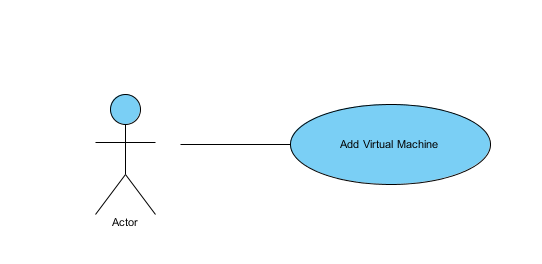
\includegraphics{images/usecase}
			
%	\section{SOFTWARE SYSTEM ATTRIBUTES}
%
%	  {\bf Performance}
%	  \\	  
%	  
%	    Performance is an indication of the responsiveness of a system to execute any action within a 
%	    given time interval. It can be measured in terms of latency or throughput. Latency is the time 
%	    taken to respond to any event. Throughput is the number of events that take place within a given amount of time.
%	    \\\\	    
%	 {\bf Reliability}
%	 \\
%	  
%	    Reliability is the ability of a system to remain operational over time. Reliability is measured as 
%	    the probability that a system will not fail to perform its intended functions over a specified time interval.
%	    \\\\	
%	  {\bf Availability}
%	  \\
%	  
%	    Availability defines the proportion of time that the system is functional and working. It can be measured 
%	    as a percentage of the total system downtime over a predefined period. Availability will be affected by 
%	    system errors, infrastructure problems, malicious attacks, and system load.
%	    \\\\
%	  {\bf Security}
%	  \\
%	  
%	    Security is the capability of a system to prevent malicious or accidental actions outside of the designed 
%	    usage, and to prevent disclosure or loss of information. A secure system aims to protect assets and prevent 
%	    unauthorized modification of information.
%	    \\\\\\\\
%	  {\bf Maintainability}
%	  \\
%	  
%	    Maintainability is the ability of the system to undergo changes with a degree of ease. These changes could 
%	    impact components, services, features, and interfaces when adding or changing the functionality, fixing 
%	    errors, and meeting new business requirements.
%	    \\\\
%	  {\bf Portability}
%	  \\
%	  
%	    Portability in high-level computer programming is the usability of the same software in different environments. 
%	    The prerequirement for portability is the generalized abstraction between the application logic and system 
%	    interfaces. When software with the same functionality is produced for several computing platforms, portability
%	    is the key issue for development cost reduction.
%
%

\end{document}
